\newpage % Rozdziały zaczynamy od nowej strony.
\section{Opis teoretyczny rozwiązania}
\par W rozdziale przedstawione zostaną wszystkie założenia teoretyczne niezbędne do pełnego zrozumienia przedmiotu pracy i późniejszej interpretacji uzyskanych rezultatów. Na początku przedstawiona zostanie idea regulacji predykcyjnej wraz z algorytmem DMC oraz obiektem regulacji, który zostanie użyty w trakcie eksperymentów. W tej części pracy przydatne były opracowania \cite{stp2009} oraz \cite{tatjewski2016}. Następnie omówię architekturę sztucznej sieci neuronowej wraz z opisem funkcji aktywacji i strategią uczenia. Istotnym działem z punktu widzenia niniejszej pracy jest opis algorytmu OBD czyli metody upraszczania sieci neuronowej wykorzystanej w trakcie eksperymentów. Na końcu omówię strategię zastosowaną w trakcie wykonanych eksperymentów.

\subsection{Regulacja Predykcyjna}
\par Regulacja predykcyjna uznawana jest za jedną z zaawansowanych technik regulacji, które to zastąpiły uprzednio powszechnie stosowane regulatory PID. Dla wielowymiarowych i skomplikowanych procesów, regulacja w oparciu o identyfikacje jednego punktu charakterystyki obiektu, jak to wygląda w regulatorze PID, może okazać się nieefektywna. Rozwiązaniem jest tutaj wykorzystanie zasady przesuwanego horyzontu i wyznaczanie w każdej chwili \(kT\), gdzie T oznacza okres próbkowania, sekwencji przyszłych wartości sygnału sterującego. Idea każdego z algorytmów regulacji predykcyjnej polega na wyznaczeniu w każdej iteracji wektora przyrostów sygnału sterującego.
 
\begin{equation}
\Delta U(k) \, = \, [\Delta u(k|k)\quad \Delta u(k+1|k)\quad \Delta u(k+2|k)\quad ... \quad \Delta u(k + N_u - 1|k)]^T
\end{equation}

gdzie przez \(N_u\) oznaczamy horyzont sterowania, a notacja \(\Delta u(k+p|k\) oznacza przyrost sygnału sterującego obliczony w chwili \(k\), który ma być wykorzystany do sterowania w chwili \(k+p\). W istocie jednak do sterowania wykorzystuje się tylko pierwszą wartość wyznaczanego wektora i prawo regulacji w kolejnych iteracjach przyjmuje postać

\begin{equation}
u(k) \, = \, u(k|k) \, = \, \Delta u(k|k) + u(k-1)
\end{equation}

\subsubsection{Algorytm DMC}
Główna idea algorytmu DMC (Dynamic Matrix Control), przedstawionego w \cite{dmc1979}, opiera się na wykorzystaniu modelu odpowiedzi skokowej do predykcji. Algorytm DMC identyfikuje dynamikę obiektu regulacji za pomocą dyskretnych odpowiedzi skokowych, które są reakcją wyjścia w kolejnych okresach próbkowania na jednostkowy skok sygnału sterującego. Na rysunku 3.1. przedstawiono przykładową odpowiedź skokową obiektu regulacji, który to opisany zostanie w kolejnym podrozdziale. Następnie tak wyznaczona odpowiedzi skokowa obiektu \(\{s_1,\, s_2,\, s_3,\, ...\, s_D \}\) wykorzystywana jest w algorytmie DMC do wyznaczenia najbardziej optymalnych wartości sterowania. Wielkość \(D\) oznacza horyzont dynamiki obiektu i powinna zostać dobrana eksperymentalnie do takiej wartości po której wyjście obiektu ulega stabilizacji. 
\begin{figure}[!h]
    \label{fig:Odpowiedz-skokowa}
    \centering 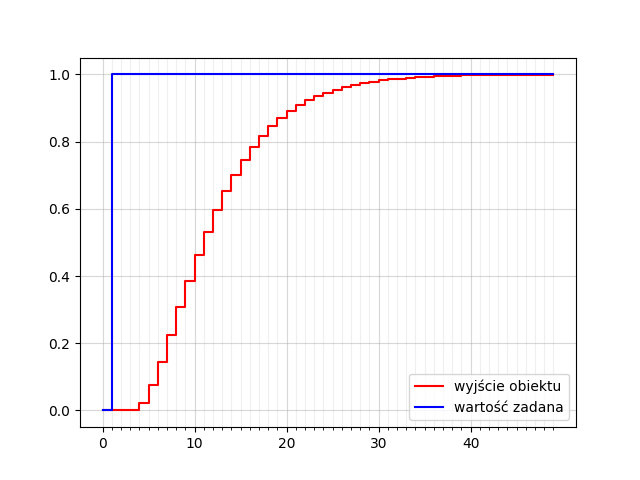
\includegraphics[width=0.5\linewidth]{Odpowiedz_skokowa.png}
    \caption{Regulacja DMC dla wybranego obiektu}
\end{figure}

\par W każdej iteracji wektor (1) wyznaczany jest w wyniku minimalizacji wskaźnika jakości, który zapisany w formie wektorowo-macierzowej przyjmuje postać
\begin{equation}
J(k) \, = \, \left\| Y^{zad}(k) - \hat{Y}(k) \right\|_{\bm{\Psi}}^2 \,+ \,\left\| \Delta U(k) \right\|_{\bm{\Lambda}}^2
\end{equation}
gdzie wektory wartości zadanej \( Y^{zad}(k) \) oraz prognozowanej trajektorii wyjścia \( \hat{Y}(k) \) o długości \( N \) będącej horyzontem predykcji definiowane są w następujący sposób
\begin{equation}
Y^{zad}(k) =
	 \begin{bmatrix}
		y^{zad}(k+1|k) \\
		\vdots \\
		y^{zad}(k+N|k)
	\end{bmatrix} , \quad
\hat{Y}(k) = 
	\begin{bmatrix}
		\hat{y}(k+1|k) \\
		\vdots \\
		\hat{y}(k+N|k)
	\end{bmatrix}
\end{equation}
macierze \( \Lambda\) oraz \( \Psi\) są macierzami diagonalnymi, a w większości przypadków przyjmują postać macierzy identyczności i takie również założenie przyjęte zostało w tej pracy. 
\par Następnie korzystając z przekształceń szczegółowo omówionych w \cite{stp2009} zapisujemy funkcję kryterialną w postaci
\begin{equation}
J(k) \, = \, \left\| Y^{zad}(k) - Y(k) - \bm{M}^P \Delta U^P(k) - \bm{M} \Delta U(k) \right\|_{\bm{\Psi}}^2 \,+ \,
\left\| \Delta U(k) \right\|_{\bm{\Lambda}}^2
\end{equation}
gdzie macierz \(M \) o wymiarowości \( N \times N_u \) ma strukturę
\begin{equation}
\bm{M} = 
	\begin{bmatrix}
		s_1 & 0 & \cdots & 0 \\
		s_2 & s_1 & \cdots & 0 \\
		\vdots & \vdots & \ddots & \vdots \\
		s_N & s_{N-1} & \cdots & s_{N-N_u+1}
	\end{bmatrix}
\end{equation}, 
macierz \(M^P \) o wymiarowości \( N \times (D-1) \) 
\begin{equation}
\bm{M^P} = 
	\begin{bmatrix}
		s_2 - s_1 & s_3 - s_2 & \cdots & s_D - s_{D-1} \\
		s_3 - s_1 & s_4 - s_2 & \cdots & s_{D+1} - S_{D-1}  \\
		\vdots & \vdots & \ddots & \vdots \\
		s_{N+1} - s_1 & s_{N+2} - s_2 & \cdots & s_{N+D-1} - s_{D-1}
	\end{bmatrix}
\end{equation}, 
natomiast wektor \( \Delta U^P(k) \) zawiera przeszłe \(D-1\) wartości zamian sygnału sterującego \(\Delta u(k-i)\). 

\par Zauważając, że funkcja jest ściśle wypukła, przyrównujemy do zera wektor gradientu funkcji i otrzymujemy wektor optymalnych przyrostów sterowania
\begin{equation}
\Delta U(k) \, = \, (\bm{M}^T\bm{\Psi}\bm{M}+\bm{\Lambda})^{-1}\bm{M}^T\bm{\Psi}(Y^{zad}(k) - Y(k) - \bm{M}^P \Delta U^P(k))
\end{equation}, 
gdzie początkową część możemy zapisać w formie 
\begin{equation}
\bm{K} \, = \, (\bm{M}^T\bm{\Psi}\bm{M}+\bm{\Lambda})^{-1}\bm{M}^T\bm{\Psi}
\end{equation}
i macierz \( \bm{K}\) jest o wymiarowości \( N_u \times N \) i wyznacza jest jednokrotnie w trakcie projektowania algorytmu. Równanie (8) jest podstawą działania algorytmu i posłuży do bezpośredniej implementacji.  

\subsubsection{Obiekt regulacji}
Aby przeprowadzić niezbędne eksperymenty i dokonać porównania różnych regulatorów niezbędne jest wybranie i zaimplementowanie obiektu regulacji. W niniejszej pracy w roli obiektu wykorzystany zostanie człon inercyjny drugiego rzędu z opóźnieniem. Wybrany układ najłatwiej przedstawić w postaci równania różnicowego 

\begin{equation}
y(k) \, = \, b_1u(k-T_d-1) + b_2u(k=T_d-2)-a_1y(k-1)-a_2y(k-2)
\end{equation}
gdzie 
\begin{align*}
a_1 \, &= \, -\alpha_1 -\alpha_2 \\
a_2 \, &= \, \alpha_1\alpha_2 \\
\alpha_1 \, &= \, e^{-\frac{1}{T_1}} \\
\alpha_2 \, &= \, e^{-\frac{1}{T_2}} \\
b_1 \, &= \, \frac{K}{T_1 - T_2}[T_1(1-\alpha_1)-T_2(1-\alpha_2)] \\
b_2 \, &= \, \frac{K}{T_1 - T_2}[\alpha_1 T_2(1-\alpha_2)-\alpha_2 T_1(1-\alpha_1)]
\end{align*}

\par Dzięki takiej prezentacji i implementacji ogólnej klasy układu regulacji mamy możliwość identyfikacji poszczególnych układów poprzez cztery parametry \( T_1, \, T_2, \, K, \, T_d \). Jest to istotna własność dzięki, której w łatwy sposób można dokonywać modyfikacji obiektu i sprawdzać zachowanie regulatora w poszczególnych przypadkach.

\par Dla lepszego zrozumienia zagadnienia warto przyjrzeć się przebiegowi regulacji predykcyjnej DMC dla jednego wybranego układu regulacji. Eksperyment przedstawiony na rysunku 3.2 przeprowadzony został dla następujących parametrów \( T_1=5, \, T_2=4, \, K=1, \, T_d=3 \) i jest dla tego samego układ wcześniej pokazana została odpowiedź skokowa.  

\begin{figure}[!h]
    \label{fig:Regulacja-DMC}
    \centering 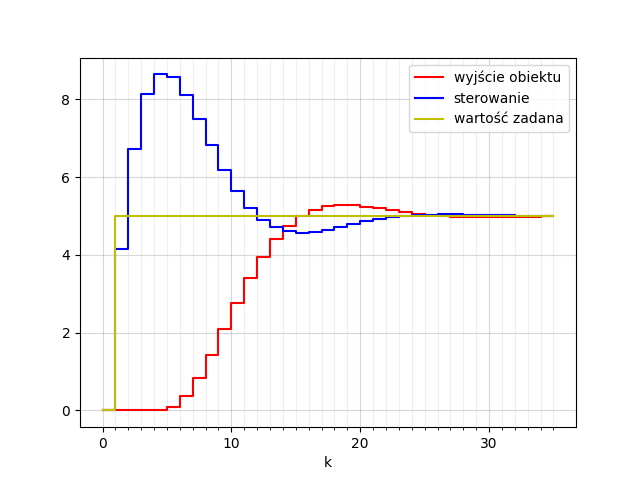
\includegraphics[width=0.5\linewidth]{Regulacja_DMC.png}
    \caption{Przykładowa odpowiedź wyjścia obiektu na jednostkowy skok sterowania}
\end{figure}

\subsection{Sztuczne Sieci Neuronowe}


\subsubsection{Architektura sieci}

\subsubsection{Algorytm OBD}

\subsection{Strategia eksperymentów}

